\section{Netzwerkschnittstelle}
Die Netzwerkschnittstelle soll die Übertragung der Daten vom Trainer zum Trainee ermöglichen. Dafür wird ein eigenes Plug-In angelegt, welches die Funktionalität der Netzwerkschnittstelle zur Verfügung stellt. Indem man die Funktionalität in ein Plug-In auslagert, ist es möglich Code hinter einem Interface zu verbergen. Dadurch ist dieser für andere Plug-Ins nicht sichtbar und die Funktionalität wird nur über eine spezifische Schnittstelle bereitgestellt. Daraus resultiert eine modulare Softwarekomponente.
Auf der Abbildung \ref{fig:NetworkInterface} hat man eine Übersicht des Moduls und über dessen Packages. Die Packages, die den Rand des Moduls berühren sind für weitere Module verwendbar.

\begin{figure}[ht]
    \centering
    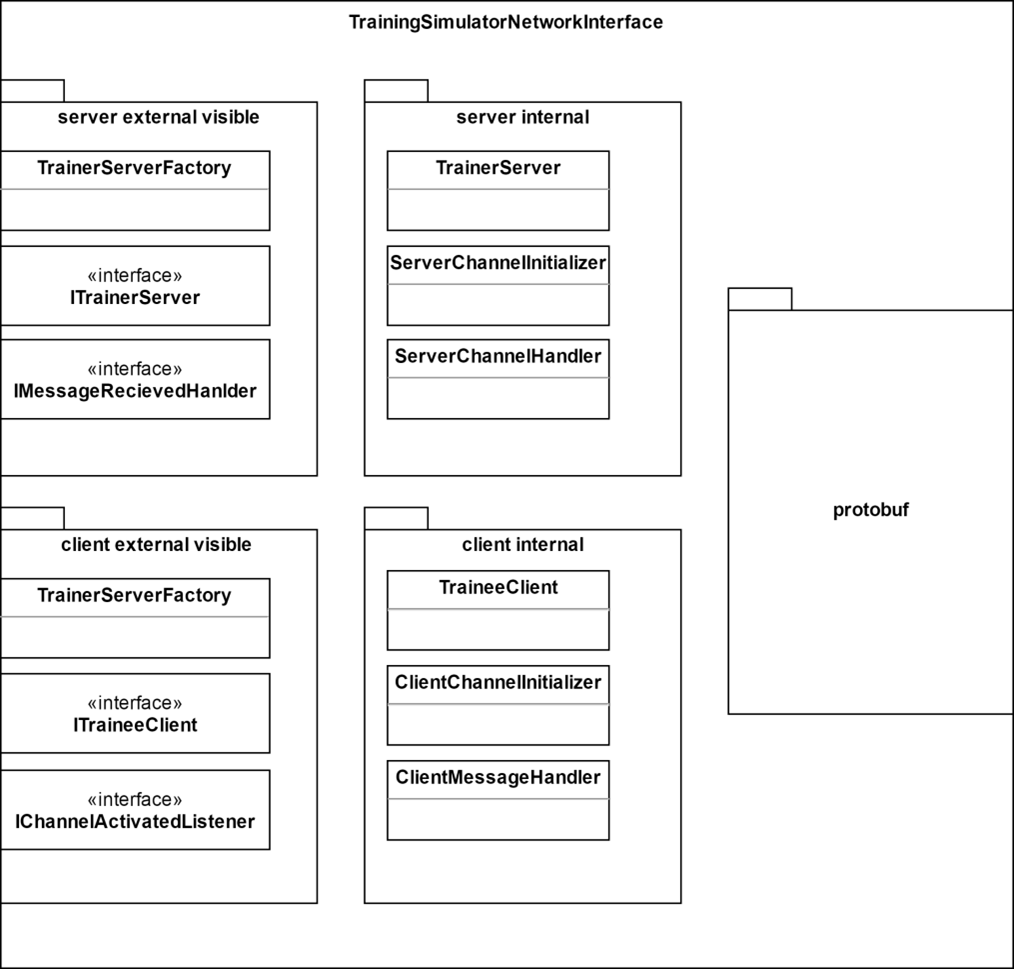
\includegraphics[width=0.9\textwidth]{content/assets/Kapitel4/NetworkInterface.png}
    \caption{Struktur des Netzwerk-Interface Moduls}
    \label{fig:NetworkInterface}
\end{figure}

\subsection{Factories}
Die Objekte, die vom \texttt{TrainingSimulatorNetworkInterface}-Modul geliefert werden sollen, sind ein \texttt{TrainerServer} vom Typ \texttt{ITrainerServer} und ein \texttt{TraineeClient} vom Typ \texttt{ITraineeClient}. Damit ein \texttt{ITrainerServer} oder ein \texttt{ITraineeClient}, einem anderen Plug-In zur Verfügung gestellt werden können, werden Factory-Klassen verwendet. Die Funktion der Factory-Klasse wird bam Beispiel der \texttt{TrainerServerFactory} erklärt.

Außerhalb des TrainingSimulatorNetworkInterface-Moduls soll die Klasse TrainerServer nicht verwendet werden. Um ein Objekt vom ITrainerServer zu erstellen benötigt man jedoch einen Konstruktor einer Klasse, die das Interface implementiert. In diesem Fall ist das die TrainerServer-Klasse. Damit ein TrainerServer-Objekt erstellt werden kann, ohne die Klasse zu verwenden, benötigt man eine Factory. Diese befindet sich im selben Modul und hat somit Zugriff auf die Klasse. Die Factory enthält die Methode getInstance(IChannelActivatedListener), die ein Objekt vom Typ ITrainerServer zurückliefert. In der Methode wird der Konstruktor des TrainerServer aufgerufen und es wird ein Objekt erstellt, welches zurückgegeben wird. Damit die Methode ausgeführt werden kann wird noch ein IChannelActivatedListener-Objekt benötigt. Dieses muss von dem Modul zur Verfügung gestellt werden, welche den ITrainerServer erzeugen will. Das Objekt stellt eine Methode bereit, welche aufgerufen wird, wenn der Server eine Verbindung zu einem Client aufgebaut hat.

Die Module, die das TrainingSimulatorNetworkInterface-Modul verwenden, kennen das Interface ITrainerServer sowie die TrainerServerFactory-Klasse, da diese vom Plug-In exportiert werden. Somit kann ein TrainerServer in einem anderen Modul über das Interface ITrainerServer verwenden, ohne dass dieses Modul die Klasse TrainerServer kennt. 

Die Factory des Clients funktioniert nach demselben Prinzip, bis auf das anstatt eines IChannelActivatedListener-Objekts, ein IMessageReceivedListener-Objekt übergeben wird. Dieses implementiert eine Methode, welche aufgerufen wird, wenn eine Nachricht empfangen wurde.